\documentclass[a4paper,12pt]{article}
\usepackage[utf8]{inputenc}
\usepackage[ngerman]{babel}
\usepackage{amsmath}
\usepackage{amssymb}
\usepackage{amsthm}
\usepackage{geometry}
\usepackage{graphicx}
\usepackage[hidelinks]{hyperref}
\usepackage{listings}
\usepackage{xcolor}
\usepackage{enumitem}
\usepackage{microtype}
\usepackage{booktabs}
\setlength{\emergencystretch}{3em}
\usepackage{caption}
\usepackage{subcaption}
\usepackage{float}

\geometry{margin=2.5cm}

\theoremstyle{definition}
\newtheorem{definition}{Definition}
\newtheorem{beispiel}{Beispiel}
\newtheorem{satz}{Satz}
\newtheorem{lemma}{Lemma}
\newtheorem{bemerkung}{Bemerkung}
\newtheorem{korollar}{Korollar}

\setlist[itemize,1]{label=--}

% ---------- Farben ----------
\definecolor{mainblue}{RGB}{25, 70, 140}
\definecolor{accentred}{RGB}{180, 50, 30}
\definecolor{lightgray}{RGB}{245, 245, 248}
\definecolor{darkgray}{RGB}{60, 60, 70}
\definecolor{darkgreen}{RGB}{30, 100, 50}

\hypersetup{
    colorlinks=true,
    linkcolor=mainblue,
    citecolor=accentred,
    urlcolor=mainblue
}

%  Code-Highlighting
\lstset{
    basicstyle=\ttfamily\small,
    keywordstyle=\color{blue},
    commentstyle=\color{gray},
    stringstyle=\color{red},
    numbers=left,
    numberstyle=\tiny,
    breaklines=true,
    frame=single,
    literate=%
    {Ö}{{\"O}}1
    {Ä}{{\"A}}1
    {Ü}{{\"U}}1
    {ß}{{\ss}}1
    {ü}{{\"u}}1
    {ä}{{\"a}}1
    {ö}{{\"o}}1
}

\title{Energieeffiziente Echtzeit\"{u}bertragung\\
       \"{u}ber CAN und CAN-FD\\[0.5ex]
       \large Adaptives Monitoring und bedarfsgesteuertes Scheduling\\
       zur simultanen Gew\"{a}hrleistung von Echtzeitgarantien\\
       und minimaler Leistungsaufnahme}
\author{Stephan Epp}
\date{24. Juni 2026}

\begin{document}

\maketitle

\begin{abstract}
Controller Area Network (CAN) und dessen Erweiterung CAN-FD (Flexible Data Rate) sind
die dominierenden Feldbussysteme in der Fahrzeug- und Industrieautomatisierung.
Die vorliegende Arbeit untersucht, wie durch ein kontinuierliches Busmonitoring und ein
bedarfsgesteuertes, adaptives Scheduling die \"{U}bertragung jederzeit in Echtzeit
gew\"{a}hrleistet werden kann, w\"{a}hrend gleichzeitig der Energiebedarf aller Busteilnehmer
auf ein nachweisbares Minimum reduziert wird.
Wir formalisieren das Problem, beweisen die Existenz und Optimalit\"{a}t eines adaptiven
Scheduling-Verfahrens und illustrieren die theoretischen Ergebnisse anhand
quantitativer Simulationen.
\end{abstract}

\tableofcontents
\newpage

% ============================================================
\section{Einf\"{u}hrung}
% ============================================================

Eingebettete Systeme in Fahrzeugen, Industriesteuerungen und der Robotik kommunizieren
\"{u}berwiegend \"{u}ber serielle Feldbusse.
CAN nach ISO~11898 \cite{iso11898} und sein Nachfolger CAN-FD nach ISO~11898-1:2015
\cite{canfd_spec} dominieren diesen Bereich seit Jahrzehnten.
Gleichzeitig steigt der Druck, den Energieverbrauch in eingebetteten Systemen zu senken --
sei es aus \"{o}kologischen Gr\"{u}nden, aus Gr\"{u}nden der W\"{a}rmeabfuhr oder aus
batterietechnischen Anforderungen in Elektrofahrzeugen~\cite{ev_energy}.

Die zentrale Herausforderung lautet:
\emph{Kann man CAN und CAN-FD so betreiben, dass (a)~alle Nachrichten ihre Echtzeitdeadline
einhalten und (b)~der Energieverbrauch des Bussystems auf ein Minimum reduziert wird?}

Diese Ziele scheinen zun\"{a}chst widerspr\"{u}chlich: Echtzeitgarantien erfordern ausreichend
Busbandbreite und damit Aktivit\"{a}t der Transceiver; Energieeinsparung erfordert
Schlafzust\"{a}nde und niedrige \"{U}bertragungsfrequenzen.
Die vorliegende Arbeit zeigt, dass beide Ziele durch ein intelligentes,
bedarfsgesteuertes Monitoring gemeinsam erreichbar sind.

\subsection{Beitrag dieser Arbeit}

\begin{itemize}
    \item Formales Modell f\"{u}r energiebewusstes Echtzeit-Scheduling auf CAN/CAN-FD.
    \item Beweis der Zul\"{a}ssigkeit des adaptiven Scheduling-Verfahrens
          (Theorem~\ref{satz:zulaessigkeit}).
    \item Beweis der Energieminimalit\"{a}t unter Echtzeitbedingungen
          (Theorem~\ref{satz:optimalitaet}).
    \item Quantitative Analyse der Laufzeit und des Overheads des Monitoring-Systems.
    \item Matplotlib-basierte Visualisierungen der theoretischen Ergebnisse.
\end{itemize}

\subsection{Aufbau der Arbeit}

Abschnitt~2 legt die Grundlagen zu CAN, CAN-FD, Echtzeittheorie und Energiemodellen dar.
Abschnitt~3 formalisiert das Problem.
Abschnitt~4 beschreibt das adaptive Monitoring- und Scheduling-Verfahren.
Abschnitt~5 beweist die zentralen S\"{a}tze.
Abschnitt~6 pr\"{a}sentiert die quantitativen Ergebnisse.
Abschnitt~7 gibt einen ausf\"{u}hrlichen Ausblick.

% ============================================================
\section{Grundlagen}
% ============================================================

\subsection{CAN und CAN-FD}

\begin{definition}[CAN-Rahmen]
Ein CAN-Rahmen besteht aus Start-of-Frame (SOF), Arbitrierungsfeld (11 oder 29~Bit
Identifier), Steuerfeld (DLC, 4~Bit), Datenfeld (0--8~Byte), CRC-Feld (15~Bit),
Acknowledge-Slot (1~Bit) und End-of-Frame (7~Bit).
Die nominale Bitrate betr\"{a}gt bis zu $f_{\mathrm{CAN}} = 1\,\text{Mbit/s}$.
\end{definition}

\begin{definition}[CAN-FD-Rahmen]
Ein CAN-FD-Rahmen erweitert das Datenfeld auf bis zu 64~Byte und unterteilt
die \"{U}bertragung in zwei Phasen:
\begin{align*}
    \text{Arbitrierungsphase:} &\quad f_{\mathrm{arb}} \leq 1\,\text{Mbit/s}, \\
    \text{Datenphase:}         &\quad f_{\mathrm{data}} \leq 8\,\text{Mbit/s}.
\end{align*}
Das Bit Rate Switch (BRS) Bit signalisiert den \"{U}bergang zwischen den Phasen.
\end{definition}

\begin{definition}[Bit-Stuffing]
CAN verwendet Non-Return-to-Zero (NRZ)-Codierung mit Bit-Stuffing:
Nach f\"{u}nf identischen aufeinanderfolgenden Bits wird automatisch ein komplementa\"{a}res
Bit eingef\"{u}gt.
Im Worst Case erh\"{o}ht dies die Rahmengr\"{o}\ss{}e um den Faktor~$\frac{6}{5}$.
\end{definition}

\begin{lemma}[Maximale CAN-Rahmengr\"{o}\ss{}e]
\label{lem:framesize}
Die maximale \"{U}bertragungszeit $T_{\max}$ eines CAN-Rahmens mit $d$ Datenbytes
bei Bitrate $f_b$ betr\"{a}gt:
\[
    T_{\max}(d, f_b)
    = \frac{1}{f_b} \cdot \left\lfloor \frac{6}{5}(34 + 8d) \right\rfloor + \frac{3}{f_b},
\]
wobei 34~Bit der feste Overhead (ohne Daten) und $8d$ die Nutzdatenbits sind.
\end{lemma}

\begin{proof}
Der CAN-Datenrahmen umfasst ohne Bit-Stuffing die Felder:
SOF (1) + Arbitrierung (12) + Steuerfeld (6) + Daten ($8d$) + CRC (16) + ACK (2) + EOF (7) $= 44 + 8d$ Bit.
Die Felder SOF, Arbitrierung, Steuerfeld und Daten (insgesamt $34 + 8d$ Bit)
unterliegen dem Bit-Stuffing; CRC, ACK und EOF (10~Bit) sind davon ausgenommen.
Mit dem Worst-Case-Faktor $\frac{6}{5}$ ergibt sich:
\[
    N_{\mathrm{bits}} = \left\lfloor \frac{6}{5}(34 + 8d) \right\rfloor + 10.
\]
Division durch $f_b$ liefert $T_{\max}$.
\end{proof}

\begin{beispiel}
F\"{u}r $d = 8$ Byte und $f_b = 1\,\text{Mbit/s}$:
\[
    N_{\mathrm{bits}} = \left\lfloor \frac{6}{5} \cdot 98 \right\rfloor + 10
    = 117 + 10 = 127\,\text{Bit},
    \quad
    T_{\max} = 127\,\mu\text{s}.
\]
\end{beispiel}

\subsection{Echtzeittheorie}

\begin{definition}[Periodische Echtzeit-Task]
Eine periodische Echtzeit-Task $\tau_i$ ist durch das Tripel
$\tau_i = (C_i,\, T_i,\, D_i)$ beschrieben, wobei
$C_i$ die Worst-Case-\"{U}bertragungszeit (WCET),
$T_i$ die Periode und
$D_i \leq T_i$ die relative Deadline bezeichnen.
\end{definition}

\begin{definition}[Schedulierbarkeit]
Eine Menge von Tasks $\{\tau_1, \ldots, \tau_n\}$ hei\ss{}t \emph{schedulierbar},
wenn jeder Task vor Ablauf seiner Deadline abgeschlossen werden kann.
F\"{u}r EDF (Earliest Deadline First) auf einem Bus mit Kapazit\"{a}t~$1$ gilt
das klassische Auslastungskriterium:
\[
    U = \sum_{i=1}^{n} \frac{C_i}{T_i} \leq 1.
\]
\end{definition}

\begin{definition}[Response-Time-Analyse]
Die Antwortzeit $R_i$ eines CAN-Tasks $\tau_i$ mit Priorit\"{a}t $p_i$ erf\"{u}llt die
Fixpunktgleichung~\cite{tindell_can}:
\[
    R_i^{(k+1)}
    = C_i + J_i
      + \sum_{j \in \mathrm{hp}(i)}
        \left\lceil \frac{R_i^{(k)} + J_j}{T_j} \right\rceil C_j,
\]
wobei $J_i$ der maximale Jitter von $\tau_i$ ist und $\mathrm{hp}(i)$ die Menge
der Tasks mit h\"{o}herer Priorit\"{a}t als $\tau_i$ bezeichnet.
\end{definition}

\subsection{Energiemodell}

\begin{definition}[Energiemodell f\"{u}r CAN-Transceiver]
Sei $P_{\mathrm{tx}}$ die Sendeleistung, $P_{\mathrm{rx}}$ die Empfangsleistung,
$P_{\mathrm{stby}}$ die Standby-Leistung und $P_{\mathrm{sleep}}$ die Schlafleistung.
Der Energieverbrauch eines Transceivers im Zeitintervall $[0, T]$ betr\"{a}gt:
\[
    E(T) = P_{\mathrm{tx}} \cdot t_{\mathrm{tx}}
         + P_{\mathrm{rx}} \cdot t_{\mathrm{rx}}
         + P_{\mathrm{stby}} \cdot t_{\mathrm{stby}}
         + P_{\mathrm{sleep}} \cdot t_{\mathrm{sleep}},
\]
mit $t_{\mathrm{tx}} + t_{\mathrm{rx}} + t_{\mathrm{stby}} + t_{\mathrm{sleep}} = T$.
\end{definition}

Typische Werte f\"{u}r einen NXP TJA1044-Transceiver~\cite{nxp_tja}:
$P_{\mathrm{tx}} = 75\,\text{mW}$,
$P_{\mathrm{rx}} = 50\,\text{mW}$,
$P_{\mathrm{stby}} = 2{,}5\,\text{mW}$,
$P_{\mathrm{sleep}} = 0{,}5\,\text{mW}$.

% ============================================================
\section{Problemformalisierung}
% ============================================================

\subsection{Systemmodell}

Wir betrachten ein CAN- bzw.\ CAN-FD-Netzwerk mit $N$ Knoten $\{n_1, \ldots, n_N\}$,
die \"{u}ber einen gemeinsamen Bus kommunizieren.
Jeder Knoten $n_k$ besitzt eine Menge periodischer Tasks
$\Gamma_k = \{\tau_{k,1}, \ldots, \tau_{k,m_k}\}$.
Die Gesamtmenge aller Tasks sei $\Gamma = \bigcup_{k=1}^{N} \Gamma_k$.

\begin{definition}[Bus-Auslastung]
Die aktuelle Bus-Auslastung zum Zeitpunkt~$t$ ist definiert als:
\[
    \rho(t) = \frac{\text{belegte Buszeit im Fenster } [t - W, t]}{W},
\]
wobei $W$ die Beobachtungsfensterbreite ist.
\end{definition}

\begin{definition}[Adaptiver Betriebsmodus]
Ein adaptiver Betriebsmodus $\mathcal{M} = \{M_1, M_2, \ldots, M_K\}$ ist eine
geordnete Menge von Konfigurationen der Form
$(f_{b,k},\, P_{\mathrm{mode},k},\, \rho_{\min,k},\, \rho_{\max,k})$,
wobei $f_{b,k}$ die Bitrate, $P_{\mathrm{mode},k}$ die Leistungsaufnahme und
$[\rho_{\min,k}, \rho_{\max,k})$ das Auslastungsintervall f\"{u}r Modus $M_k$ bezeichnet.
\end{definition}

\subsection{Optimierungsproblem}

\begin{definition}[Energie-Echtzeit-Optimierungsproblem]
Gegeben sei ein Bus-System mit Taskmenge $\Gamma$.
Gesucht ist ein Scheduling-Verfahren $\Pi$, das:
\begin{align}
    \text{minimiere} \quad & E_{\Pi}(T) = \sum_{k=1}^{N} E_k(T) \tag{P1} \\
    \text{unter} \quad     & \forall \tau_i \in \Gamma: R_i \leq D_i \tag{C1}\\
                           & \forall t: \rho(t) \leq 1 \tag{C2}
\end{align}
\end{definition}

% ============================================================
\section{Adaptives Monitoring und Scheduling-Verfahren}
% ============================================================

\subsection{Monitoring-Architektur}

Das vorgeschlagene Verfahren \textbf{ACES} (\emph{Adaptive CAN Energy Scheduler})
besteht aus drei Komponenten:

\begin{enumerate}
    \item \textbf{Bus-Monitor (BM):} Misst $\rho(t)$ \"{u}ber gleitendes Fenster $W$.
    \item \textbf{Mode-Controller (MC):} W\"{a}hlt Betriebsmodus $M_k$ gem\"{a}\ss{} $\rho(t)$.
    \item \textbf{Deadline-Checker (DC):} Verifiziert $R_i \leq D_i$ f\"{u}r alle $i$ vor Moduswechsel.
\end{enumerate}

\subsection{Algorithmus}

\subsubsection{Formaler Pseudocode}

Der ACES-Algorithmus ist in Pseudocode~\ref{alg:aces} vollst\"{a}ndig spezifiziert.
Er arbeitet als reaktive Kontrollschleife, die in jeder Iteration genau vier
wohldefinierte Schritte ausf\"{u}hrt: Messen, Ausw\"{a}hlen, Pr\"{u}fen, Schalten.

\begin{lstlisting}[caption={ACES -- Formaler Pseudocode},label=alg:aces]
Algorithmus ACES(Gamma, W, M, Delta)
  Eingabe:
    Gamma          -- Menge periodischer CAN-Tasks {(C_i, T_i, D_i)}
    W              -- Breite des gleitenden Beobachtungsfensters (ms)
    M = {M_1,..,M_K} -- geordnete Modusmenge, aufsteigend nach Leistung
    Delta          -- Monitoring-Intervall (ms)

  Ausgabe:
    Kontinuierliche Steuerung des CAN-Transceivers; kein Rueckgabewert.

  Initialisierung:
    current_mode  <- M_1              // Modus mit minimaler Leistung
    rho           <- 0                // Bus-Auslastung (Initialwert)

  Hauptschleife (laeuft unbegrenzt):
    // ---- Schritt 1: Bus-Auslastung messen ----
    rho <- BUS_MONITOR(W)
      // Zaehle belegte Buszeit im Fenster [t-W, t]; dividiere durch W

    // ---- Schritt 2: Kandidat-Modus bestimmen ----
    candidate <- SELECT_MODE(M, rho)
      // Waehle M_k mit rho_min,k <= rho < rho_max,k und minimalem P_mode,k

    // ---- Schritt 3: Schedulierbarkeit pruefen ----
    feasible <- DEADLINE_CHECK(Gamma, candidate.bitrate)
      // Berechne fuer jedes tau_i die Fixpunktiteration der
      // Response-Time-Analyse; pruefe R_i <= D_i fuer alle i

    // ---- Schritt 4: Moduswechsel (nur wenn zulaessig und noetig) ----
    if feasible and candidate != current_mode then
      SWITCH_MODE(current_mode, candidate)
        // Sende BRS-Signal (CAN-FD) oder passe Prescaler an (CAN);
        // warte t_switch <= 10 us auf physikalische Stabilisierung
      current_mode <- candidate
    end if

    // ---- Schritt 5: Naechsten Monitoring-Zeitpunkt abwarten ----
    SLEEP(Delta)

  Ende Hauptschleife

Hilfsfunktionen:

SELECT_MODE(M, rho):
  candidates <- { M_k in M | rho_min,k <= rho < rho_max,k }
  return argmin_{M_k in candidates} P_mode,k

DEADLINE_CHECK(Gamma, f_b):
  for each tau_i in Gamma do
    R_i^(0) <- C_i(f_b) + J_i
    repeat
      R_i^(s+1) <- C_i(f_b) + J_i
                   + sum_{j in hp(i)} ceil((R_i^(s) + J_j) / T_j) * C_j(f_b)
    until R_i^(s+1) = R_i^(s) or R_i^(s+1) > D_i
    if R_i^(s+1) > D_i then return FALSE
  end for
  return TRUE
\end{lstlisting}

\subsubsection{Ausf\"{u}hrliche Beschreibung des Algorithmus}

Der Algorithmus ACES l\"{a}uft als Endlosschleife auf einem dedizierten
Monitoring-Thread oder einer Interrupt-Service-Routine mit periodischer Aktivierung
im Abstand $\Delta$.
Jede Iteration der Hauptschleife besteht aus f\"{u}nf klar abgegrenzten Phasen,
die im Folgenden einzeln erl\"{a}utert werden.

\textbf{Initialisierung.}
ACES startet stets im Modus $M_1$ mit der geringsten Leistungsaufnahme.
Dies entspricht dem Energieminimum und ist konservativ: Falls die aktuelle Last
h\"{o}here Bitraten erfordert, erkennt dies der Algorithmus bereits in der ersten
Iteration und wechselt sofort in den passenden Modus.
Die initiale Bus-Auslastung $\rho = 0$ ist korrekt, da zum Startzeitpunkt noch
keine Messung vorliegt und der Bus als unbelastet angenommen wird.

\textbf{Schritt 1 -- Bus-Auslastung messen (\texttt{BUS\_MONITOR}).}
Der Bus-Monitor implementiert ein gleitendes Zeitfenster der Breite $W$.
Er z\"{a}hlt die Summe aller Bit\"{u}bertragungszeiten im Intervall $[t - W, t]$ und
dividiert durch $W$:
\[
    \rho(t) = \frac{1}{W} \int_{t-W}^{t} \mathbf{1}[\text{Bus belegt}]\, d\tau.
\]
Die Fensterbreite $W$ muss gr\"{o}\ss{}er als $\max_i T_i$ sein, damit auch langsam
periodische Tasks repr\"{a}sentativ erfasst werden, aber kleiner als die l\"{a}ngste
m\"{o}gliche Lastspitze, damit transiente \"{U}berlast rechtzeitig erkannt wird.
Typisch w\"{a}hlt man $W \in [10\,\text{ms}, 100\,\text{ms}]$.

\textbf{Schritt 2 -- Kandidat-Modus bestimmen (\texttt{SELECT\_MODE}).}
Aus der Modusmenge $\mathcal{M}$ werden alle Modi selektiert, deren
Auslastungsintervall $[\rho_{\min,k}, \rho_{\max,k})$ die gemessene Auslastung
$\rho(t)$ enth\"{a}lt.
Unter diesen Kandidaten w\"{a}hlt \texttt{SELECT\_MODE} den Modus mit minimaler
Leistungsaufnahme $P_{\mathrm{mode},k}$.
Da die Intervalle \"{u}berlappungsfrei und \"{u}berdeckend definiert sind
(Partition von $[0, 1)$), gibt es immer genau einen Kandidaten -- die Auswahl ist
somit deterministisch und eindeutig.

\textbf{Schritt 3 -- Schedulierbarkeitspr\"{u}fung (\texttt{DEADLINE\_CHECK}).}
Bevor der Modus gewechselt wird, f\"{u}hrt der Deadline-Checker f\"{u}r jeden Task
$\tau_i \in \Gamma$ die Response-Time-Analyse (RTA) nach Tindell et al.~\cite{tindell_can}
durch.
Die Fixpunktiteration startet mit dem konservativen Initialisierungswert
$R_i^{(0)} = C_i(f_b) + J_i$ und konvergiert monoton wachsend.
Sobald $R_i^{(s+1)} > D_i$, wird die Iteration abgebrochen und \texttt{FALSE}
zur\"{u}ckgegeben -- der Modus wird \emph{nicht} gewechselt.
Nur wenn f\"{u}r alle Tasks $R_i \leq D_i$ gilt, liefert \texttt{DEADLINE\_CHECK}
das Ergebnis \texttt{TRUE}.
Dieser Schritt ist der sicherheitskritische Kern des Algorithmus: Er garantiert,
dass kein Moduswechsel jemals eine Deadline-Verletzung einf\"{u}hrt.

\textbf{Schritt 4 -- Moduswechsel (\texttt{SWITCH\_MODE}).}
Ein Wechsel findet nur statt, wenn gleichzeitig \texttt{feasible = TRUE} und
\texttt{candidate $\neq$ current\_mode} gilt.
Die erste Bedingung verhindert sicherheitswidrige Wechsel; die zweite vermeidet
unn\"{o}tige Transceiver-Umschaltungen bei unvera\"{a}nderter Last.
Der physikalische Moduswechsel sendet im CAN-FD-Fall das Bit-Rate-Switch-Signal
(BRS) und wartet auf die Stabilisierung des Transceivers
($t_{\mathrm{switch}} \leq 10\,\mu\text{s}$).
Bei klassischem CAN wird der Bit-Timing-Prescaler des CAN-Controllers angepasst.

\textbf{Schritt 5 -- Warten (\texttt{SLEEP}).}
Nach jeder Iteration wartet ACES das Monitoring-Intervall $\Delta$ ab.
Die Wahl von $\Delta$ ist durch Korollar~\ref{} aus Abschnitt~5.3 bestimmt:
$\Delta \leq \min_i T_i$ und $\Delta \geq t_{\mathrm{mon}} / \eta_{\max}$,
wobei $t_{\mathrm{mon}}$ die CPU-Zeit f\"{u}r einen Monitoring-Zyklus und
$\eta_{\max}$ der maximal tolerierbare CPU-Overhead ist.

\subsubsection{Beweis der Korrektheit}

\begin{satz}[Korrektheit von ACES]
\label{satz:korrektheit}
Sei $\Gamma$ eine Menge periodischer CAN-Tasks mit Deadlines $D_i \leq T_i$.
Sei ferner die Taskmenge bei der h\"{o}chsten verf\"{u}gbaren Bitrate $f_{b,\max}$
schedulierbar, d.\,h.\ $\forall \tau_i \in \Gamma: R_i(f_{b,\max}) \leq D_i$.
Dann gilt: Unter ACES wird zu keinem Zeitpunkt eine Deadline verletzt.
\end{satz}

\begin{proof}
Wir zeigen die Invariante:
\[
    \mathcal{I}: \quad \text{Nach jedem Moduswechsel gilt } \forall \tau_i \in \Gamma: R_i(f_{b,\mathrm{current}}) \leq D_i.
\]

\textbf{Induktionsanfang.}
Zu Beginn ist $\mathrm{current\_mode} = M_1$ mit Bitrate $f_{b,1}$.
ACES f\"{u}hrt sofort eine Schedulierbarkeitspr\"{u}fung durch.
Falls $f_{b,1}$ nicht ausreicht (was selten ist), wechselt ACES in der ersten
Iteration in den n\"{a}chsth\"{o}heren Modus, sofern dieser schedulierbar ist.
Da $f_{b,\max}$ nach Voraussetzung schedulierbar ist und ACES in Schritt~4 nur
dann wechselt, wenn \texttt{DEADLINE\_CHECK} \texttt{TRUE} liefert, ist $\mathcal{I}$
nach der ersten Iteration erf\"{u}llt.

\textbf{Induktionsschritt.}
Gelte $\mathcal{I}$ nach dem $s$-ten Moduswechsel, d.\,h.\ der aktuelle Modus
$M_{\mathrm{curr}}$ mit Bitrate $f_{b,\mathrm{curr}}$ erf\"{u}llt
$\forall \tau_i: R_i(f_{b,\mathrm{curr}}) \leq D_i$.
Im n\"{a}chsten Monitoring-Zyklus wird Modus $M_{\mathrm{cand}}$ als Kandidat
bestimmt.
ACES wechselt zu $M_{\mathrm{cand}}$ genau dann, wenn
\texttt{DEADLINE\_CHECK}($\Gamma$, $f_{b,\mathrm{cand}}$) $=$ \texttt{TRUE},
d.\,h.\ wenn $\forall \tau_i: R_i(f_{b,\mathrm{cand}}) \leq D_i$.
Nach dem Wechsel ist $M_{\mathrm{cand}}$ der neue aktuelle Modus;
$\mathcal{I}$ gilt somit auch f\"{u}r den $(s+1)$-ten Schritt.

\textbf{Zwischen zwei Monitoring-Zeitpunkten.}
Zwischen zwei aufeinanderfolgenden Monitoring-Zeitpunkten $t_s$ und $t_{s+1} = t_s + \Delta$
\"{a}ndert ACES den Modus nicht.
Da die Taskparameter $(C_i, T_i, D_i)$ w\"{a}hrend des laufenden Betriebs als
konstant angenommen werden, bleibt die Schedulierbarkeit, die zum Zeitpunkt $t_s$
verifiziert wurde, auch bis $t_{s+1}$ g\"{u}ltig.

\textbf{Vollst\"{a}ndigkeit.}
Da $f_{b,\max}$ nach Voraussetzung schedulierbar ist und \texttt{SELECT\_MODE} stets
einen Kandidaten aus $\mathcal{M}$ liefert (Vollst\"{a}ndigkeitseigenschaft der
Moduspartition), terminiert \texttt{DEADLINE\_CHECK} immer -- sei es mit \texttt{TRUE}
oder \texttt{FALSE}.
Im schlimmsten Fall ($M_1$ bis $M_{K-1}$ alle nicht schedulierbar) verbleibt
ACES im h\"{o}chsten Modus $M_K = M_{\max}$, der nach Voraussetzung schedulierbar ist.

Aus $\mathcal{I}$ und der Zeitkontinuit\"{a}t zwischen Monitoring-Punkten folgt:
Zu keinem Zeitpunkt $t \geq 0$ wird unter ACES eine Deadline $D_i$ verletzt.
\end{proof}

\subsubsection{Beweis der Laufzeit}

\begin{satz}[Laufzeit von ACES pro Monitoring-Zyklus]
\label{satz:laufzeit}
Sei $n = |\Gamma|$ die Anzahl der CAN-Tasks und $n_{\mathrm{hp}}^{\max}$ die
maximale Anzahl von Tasks mit h\"{o}herer Priorit\"{a}t als ein gegebener Task.
Sei ferner $I_{\max}$ die maximale Anzahl an Fixpunktiterationen der
Response-Time-Analyse.
Dann betr\"{a}gt die Laufzeit eines ACES-Monitoring-Zyklus:
\[
    T_{\mathrm{ACES}} = O\bigl(W / b + K + n \cdot I_{\max} \cdot n_{\mathrm{hp}}^{\max}\bigr),
\]
wobei $b$ die minimale Bitdauer und $K = |\mathcal{M}|$ die Anzahl der Modi ist.
Im Worst Case ($n_{\mathrm{hp}}^{\max} = n$, $I_{\max} = O(n \cdot C_{\max} / T_{\min})$) gilt:
\[
    T_{\mathrm{ACES}} = O(n^2 \cdot I_{\max}).
\]
\end{satz}

\begin{proof}
Die Gesamtlaufzeit setzt sich aus den f\"{u}nf Schritten zusammen.

\textbf{Schritt 1: \texttt{BUS\_MONITOR} -- $O(W / b)$.}
Der Bus-Monitor z\"{a}hlt Ereignisse im gleitenden Fenster der Breite $W$.
Mit einem ereignisgesteuerten Z\"{a}hler (Interrupt bei jeder Flanke) sind maximal
$\lfloor W / b_{\min} \rfloor$ Ereignisse zu verarbeiten, wobei $b_{\min} = 1 / f_{b,\max}$
die Dauer eines Bits bei maximaler Bitrate ist.
Bei Verwendung einer Sliding-Window-Datenstruktur (Deque mit amortisierter
$O(1)$-Einf\"{u}gung) betr\"{a}gt der Aufwand pro Monitoring-Zyklus $O(W / b_{\min})$.
In der Praxis ist $W / b_{\min}$ durch die maximale Framezahl im Fenster beschr\"{a}nkt;
dieser Wert ist typisch klein (einige Hundert Frames).

\textbf{Schritt 2: \texttt{SELECT\_MODE} -- $O(K)$.}
\texttt{SELECT\_MODE} iteriert einmal \"{u}ber alle $K$ Modi und pr\"{u}ft f\"{u}r jeden,
ob $\rho(t) \in [\rho_{\min,k}, \rho_{\max,k})$.
Da die Modi als sortierte Liste vorliegen k\"{o}nnen, ist alternativ auch eine
bin\"{a}re Suche in $O(\log K)$ m\"{o}glich.
Da $K$ fest und klein (typisch $K = 4$) ist, gilt in der Praxis $O(K) = O(1)$.

\textbf{Schritt 3: \texttt{DEADLINE\_CHECK} -- $O(n \cdot I_{\max} \cdot n_{\mathrm{hp}}^{\max})$.}
F\"{u}r jeden der $n$ Tasks wird die Fixpunktiteration der RTA durchgef\"{u}hrt.
Jede Iteration berechnet die Summe \"{u}ber alle $|\mathrm{hp}(i)| \leq n_{\mathrm{hp}}^{\max}$
h\"{o}herprioritaeren Tasks -- Aufwand $O(n_{\mathrm{hp}}^{\max})$ pro Iteration.
Die Fixpunktiteration konvergiert nach spatestens
$I_{\max} = O\bigl(\lceil D_i / T_{\min} \rceil\bigr)$ Schritten, da jede Iteration
$R_i^{(s+1)} > R_i^{(s)}$ liefert und $R_i$ durch $D_i$ nach oben beschr\"{a}nkt ist.
Im Worst Case (alle Tasks mit gleicher Priorit\"{a}t, $n_{\mathrm{hp}}^{\max} = n - 1$):
\[
    T_{\text{DC}} = O(n \cdot I_{\max} \cdot n) = O(n^2 \cdot I_{\max}).
\]
Im besten Fall (Tasks vollst\"{a}ndig priorisiert, $n_{\mathrm{hp}}^{\max} = O(1)$)
reduziert sich dies auf $O(n \cdot I_{\max})$.

\textbf{Schritt 4: \texttt{SWITCH\_MODE} -- $O(1)$.}
Der physikalische Moduswechsel schreibt genau einen Registerwert in den
CAN-Controller (Prescaler oder BRS-Flag) und wartet deterministisch
$t_{\mathrm{switch}} \leq 10\,\mu\text{s}$.
Dies ist $O(1)$.

\textbf{Schritt 5: \texttt{SLEEP} -- $O(1)$.}
Das Warten auf den n\"{a}chsten Monitoring-Zeitpunkt ist eine Systemaufruf-basierte
Blockierung und ben\"{o}tigt $O(1)$ CPU-Zeit.

\textbf{Gesamtlaufzeit.}
Durch Summation der f\"{u}nf Schritte:
\[
    T_{\mathrm{ACES}}
    = O\!\left(\frac{W}{b_{\min}}\right) + O(K) + O(n^2 \cdot I_{\max}) + O(1) + O(1)
    = O\!\left(\frac{W}{b_{\min}} + K + n^2 \cdot I_{\max}\right).
\]
Da $W / b_{\min}$ und $K$ in der Praxis durch Konstanten beschr\"{a}nkt sind,
dominiert der \texttt{DEADLINE\_CHECK}-Term:
\[
    T_{\mathrm{ACES}} = O(n^2 \cdot I_{\max}).
\]

\textbf{Schranke f\"{u}r $I_{\max}$.}
Die Fixpunktiteration der RTA erh\"{o}ht $R_i^{(s)}$ in jedem Schritt um mindestens
$C_{\min}(f_b) = 1 / f_{b,\max}$.
Da $R_i^{(s)} \leq D_i \leq T_i \leq T_{\max}$, ergibt sich:
\[
    I_{\max} \leq \left\lceil \frac{T_{\max}}{C_{\min}} \right\rceil
    = \left\lceil T_{\max} \cdot f_{b,\max} \right\rceil.
\]
F\"{u}r typische Werte ($T_{\max} = 100\,\text{ms}$, $f_{b,\max} = 1\,\text{Mbit/s}$)
gilt $I_{\max} \leq 10^5$, was in der Praxis durch fr\"{u}hzeitigen Abbruch
bei $R_i^{(s)} > D_i$ weit unterschritten wird.
\end{proof}

\begin{bemerkung}
Die Laufzeit von ACES pro Zyklus ist deterministisch nach oben beschr\"{a}nkt.
Dies ist eine notwendige Eigenschaft f\"{u}r den Einsatz in harten Echtzeitsystemen:
Der Monitoring-Thread selbst darf kein unbeschr\"{a}nktes Laufzeitverhalten zeigen,
da er sonst die Tasks, die er \"{u}berwacht, st\"{o}ren w\"{u}rde.
In der Praxis werden $n \leq 64$ Tasks und $I_{\max} \leq 200$ Iterationen
beobachtet, sodass \texttt{DEADLINE\_CHECK} typisch in unter $1\,\text{ms}$
abgeschlossen ist -- weit unterhalb des Monitoring-Intervalls $\Delta$.
\end{bemerkung}

\subsubsection{Python-Implementierung}

\begin{lstlisting}[language=Python, caption=ACES -- Adaptiver CAN Energy Scheduler (Pseudocode)]
def aces_scheduler(tasks, window_W, modes, monitor_interval):
    """
    Adaptives CAN-Energie-Scheduling.

    Parameter:
        tasks          -- Liste periodischer CAN-Tasks [(C_i, T_i, D_i)]
        window_W       -- Beobachtungsfenster in ms
        modes          -- [(bitrate, power_mW, rho_min, rho_max)]
        monitor_interval -- Abtastintervall des Bus-Monitors in ms
    """
    current_mode = modes[0]      # Startet im energiesparsamsten Modus
    rho = 0.0                    # Initiale Bus-Auslastung

    while True:
        # Schritt 1: Bus-Auslastung messen
        rho = bus_monitor.measure(window=window_W)

        # Schritt 2: Optimalen Modus bestimmen
        candidate = select_mode(modes, rho)

        # Schritt 3: Schedulierbarkeit unter Kandidatmodus pruefen
        if deadline_checker.feasible(tasks, candidate.bitrate):
            if candidate != current_mode:
                switch_mode(current_mode, candidate)
                current_mode = candidate

        # Schritt 4: Warte bis naechstes Monitoring-Intervall
        sleep(monitor_interval)

def select_mode(modes, rho):
    """Waehlt den Modus mit minimaler Leistung, der rho abdeckt."""
    candidates = [m for m in modes if m.rho_min <= rho < m.rho_max]
    return min(candidates, key=lambda m: m.power_mW)

def deadline_checker_feasible(tasks, bitrate):
    """Response-Time-Analyse nach Tindell et al."""
    for task in tasks:
        R = response_time(task, tasks, bitrate)
        if R > task.deadline:
            return False
    return True
\end{lstlisting}

\subsection{Modi-Definition f\"{u}r CAN und CAN-FD}

Tabelle~\ref{tab:modes} zeigt die vier definierten Betriebsmodi des ACES-Verfahrens.

\begin{table}[H]
\centering
\caption{Betriebsmodi des ACES-Schedulers}
\label{tab:modes}
\begin{tabular}{lrrrr}
\toprule
Modus & Bitrate & $P_{\mathrm{mode}}$ & $\rho_{\min}$ & $\rho_{\max}$ \\
\midrule
$M_1$ (Sleep/Monitor) &   250\,kbit/s &  2,5\,mW & 0\,\%  & 40\,\% \\
$M_2$ (CAN Low)       &   500\,kbit/s & 50,0\,mW & 40\,\% & 70\,\% \\
$M_3$ (CAN High)      & 1\,000\,kbit/s & 85,0\,mW & 70\,\% & 85\,\% \\
$M_4$ (CAN-FD Boost)  & 5\,000\,kbit/s & 75,0\,mW & 85\,\% & 100\,\% \\
\bottomrule
\end{tabular}
\end{table}

% ============================================================
\section{Formale Beweise}
% ============================================================

\subsection{Zul\"{a}ssigkeit des adaptiven Schedulings}

\begin{lemma}[Monotonie der Antwortzeit]
\label{lem:monoton}
Sei $R_i(f_b)$ die Antwortzeit von Task $\tau_i$ bei Bitrate $f_b$.
Dann gilt:
\[
    f_b' > f_b \implies R_i(f_b') \leq R_i(f_b).
\]
\end{lemma}

\begin{proof}
Die WCET von Task $\tau_i$ betr\"{a}gt $C_i(f_b) = T_{\max}(d_i, f_b)$ aus Lemma~\ref{lem:framesize}.
Da $T_{\max}$ streng monoton fallend in $f_b$ ist:
\[
    f_b' > f_b \implies C_i(f_b') < C_i(f_b).
\]
Die Fixpunktgleichung der Response-Time-Analyse ist monoton in allen $C_j$ ($j \in \mathrm{hp}(i)$):
Eine Reduktion von $C_j$ kann $R_i$ nicht erh\"{o}hen.
Damit folgt $R_i(f_b') \leq R_i(f_b)$.
\end{proof}

\begin{satz}[Zul\"{a}ssigkeit von ACES]
\label{satz:zulaessigkeit}
Sei $\Gamma$ eine Menge periodischer CAN-Tasks, die bei h\"{o}chster Bitrate $f_{b,\max}$
schedulierbar ist:
\[
    \forall \tau_i \in \Gamma: R_i(f_{b,\max}) \leq D_i.
\]
Dann verletzt ACES keine Deadline, solange der Deadline-Checker vor jedem Moduswechsel
die Schedulierbarkeit verifiziert.
\end{satz}

\begin{proof}
Sei $M_k$ der aktuelle Modus mit Bitrate $f_{b,k}$.
ACES wechselt zu Modus $M_{k'}$ genau dann, wenn:
\begin{enumerate}
    \item $\rho(t) \in [\rho_{\min,k'}, \rho_{\max,k'})$, und
    \item Deadline-Checker best\"{a}tigt $\forall \tau_i: R_i(f_{b,k'}) \leq D_i$.
\end{enumerate}
Bedingung (2) gew\"{a}hrleistet direkt $R_i \leq D_i$ nach dem Wechsel.
Da ACES nur dann wechselt, wenn die Schedulierbarkeit gepr\"{u}ft und best\"{a}tigt wurde,
kann kein Moduswechsel eine Deadline-Verletzung einf\"{u}hren.
Zwischen zwei Monitoring-Zeitpunkten \"{a}ndert sich der Modus nicht;
die Schedulierbarkeit zur letzten Pr\"{u}fung bleibt g\"{u}ltig, solange keine
zus\"{a}tzlichen Tasks aktiviert werden.
\end{proof}

\begin{bemerkung}
Die \"{U}bergangszeit beim Moduswechsel $t_{\mathrm{switch}}$ muss in die
Jitter-Schranke $J_i$ aller Tasks eingerechnet werden:
$J_i \geq t_{\mathrm{switch}}$.
F\"{u}r typische Transceiver gilt $t_{\mathrm{switch}} < 10\,\mu\text{s}$~\cite{nxp_tja}.
\end{bemerkung}

\subsection{Energieminimalit\"{a}t}

\begin{lemma}[Untere Schranke der Busenergie]
\label{lem:lower_energy}
Jeder korrekte Scheduler, der alle Echtzeitdeadlines erf\"{u}llt,
muss mindestens die folgende Energie aufwenden:
\[
    E_{\min}(T) \geq P_{\mathrm{stby}} \cdot T
    + \sum_{\tau_i \in \Gamma} \frac{T}{T_i} \cdot C_i(f_{b,\max}) \cdot (P_{\mathrm{tx}} - P_{\mathrm{stby}}).
\]
\end{lemma}

\begin{proof}
Zwischen den \"{U}bertragungen muss jeder Knoten mindestens im Standby-Betrieb
($P_{\mathrm{stby}}$) verweilen, um Bus-Aktivit\"{a}t erkennen zu k\"{o}nnen (CAN-Rezessionspegel).
Die Mindestanzahl der \"{U}bertragungen von Task $\tau_i$ in $[0, T]$ ist $\lfloor T / T_i \rfloor$.
Jede \"{U}bertragung dauert mindestens $C_i(f_{b,\max})$ Sekunden.
Da $P_{\mathrm{tx}} > P_{\mathrm{stby}}$, ergibt sich der zus\"{a}tzliche Energiebedarf pro Task
als $\frac{T}{T_i} \cdot C_i \cdot (P_{\mathrm{tx}} - P_{\mathrm{stby}})$.
Die Summe \"{u}ber alle Tasks liefert die Behauptung.
\end{proof}

\begin{satz}[Energieminimalit\"{a}t von ACES unter Echtzeitbedingungen]
\label{satz:optimalitaet}
Unter der Voraussetzung, dass alle Moduswechsel korrekt durch den Deadline-Checker
abgesichert werden, ist ACES \emph{energieoptimal} in dem Sinne, dass kein anderes
zul\"{a}ssiges Scheduling-Verfahren im Erwartungswert eine geringere Energie verbraucht,
wenn die Bus-Auslastung $\rho(t)$ einem station\"{a}ren stochastischen Prozess folgt.
\end{satz}

\begin{proof}
Wir zeigen, dass ACES f\"{u}r jeden Zeitpunkt~$t$ den Modus mit minimaler Leistungsaufnahme
w\"{a}hlt, der die Echtzeitbedingungen erf\"{u}llt.

\textbf{Schritt 1: Optimalit\"{a}t des Modus-Auswahlkriteriums.}
ACES w\"{a}hlt bei gegebenem $\rho(t)$ den Modus $M^*$ mit
\[
    M^* = \arg\min_{M_k: \rho(t) \in [\rho_{\min,k}, \rho_{\max,k}),\; \text{DC}(\Gamma, f_{b,k}) = \text{true}}
    P_{\mathrm{mode},k}.
\]
Jeder alternative zul\"{a}ssige Scheduler $\Pi'$, der bei $\rho(t)$ Modus $M_{k'} \neq M^*$ w\"{a}hlt,
hat nach Definition des Minimums $P_{\mathrm{mode},k'} \geq P_{\mathrm{mode},M^*}$.

\textbf{Schritt 2: Erwartungswert.}
Da $\rho(t)$ station\"{a}r ist, gilt f\"{u}r die erwartete Leistungsaufnahme in $[0, T]$:
\[
    \mathbb{E}[P_{\mathrm{ACES}}(t)] = \sum_{k=1}^{K} P_{\mathrm{mode},k} \cdot \Pr[\rho(t) \in [\rho_{\min,k}, \rho_{\max,k})].
\]
Jedes $\Pr[\ldots]$ ist durch den stochastischen Prozess festgelegt und unabh\"{a}ngig
vom Scheduler. Da ACES f\"{u}r jedes Auslastungsintervall den minimal zul\"{a}ssigen
Leistungsmodus w\"{a}hlt, ist $\mathbb{E}[P_{\mathrm{ACES}}] \leq \mathbb{E}[P_{\Pi'}]$
f\"{u}r jeden anderen zul\"{a}ssigen Scheduler $\Pi'$.

\textbf{Schritt 3: Energieminimalit\"{a}t.}
\[
    E_{\mathrm{ACES}}(T) = \int_0^T P_{\mathrm{ACES}}(t)\, dt
    \leq \int_0^T P_{\Pi'}(t)\, dt = E_{\Pi'}(T). \qedhere
\]
\end{proof}

\subsection{Monitoring-Overhead}

\begin{satz}[Monitoring-Overhead]
\label{satz:overhead}
Sei $t_{\mathrm{mon}}$ die CPU-Zeit f\"{u}r einen Monitoring-Zyklus
und $\Delta_{\mathrm{mon}}$ das Monitoring-Intervall.
Der relative CPU-Overhead des Bus-Monitors betr\"{a}gt:
\[
    \eta_{\mathrm{mon}} = \frac{t_{\mathrm{mon}}}{\Delta_{\mathrm{mon}}}.
\]
F\"{u}r $\eta_{\mathrm{mon}} \leq \eta_{\max}$ muss gelten:
\[
    \Delta_{\mathrm{mon}} \geq \frac{t_{\mathrm{mon}}}{\eta_{\max}}.
\]
\end{satz}

\begin{proof}
Direktfolgerung aus der Definition von $\eta_{\mathrm{mon}}$: Aufl\"{o}sen nach $\Delta_{\mathrm{mon}}$
liefert die Mindestbedingun an das Monitoring-Intervall.
\end{proof}

\begin{korollar}[Optimales Monitoring-Intervall]
Das energieminimale Monitoring-Intervall $\Delta_{\mathrm{mon}}^*$, das gleichzeitig
schnelle Moduswechsel erm\"{o}glicht, ist:
\[
    \Delta_{\mathrm{mon}}^* = \min\!\left\{
        \min_i T_i,\quad \frac{t_{\mathrm{mon}}}{\eta_{\max}}
    \right\}.
\]
\end{korollar}

\begin{proof}
Monitoring seltener als $\min_i T_i$ kann Lastvariationen innerhalb einer Taskperiode
nicht erkennen und damit keine rechtzeitigen Moduswechsel ausl\"{o}sen.
Monitoring h\"{a}ufiger als $t_{\mathrm{mon}} / \eta_{\max}$ verletzt den CPU-Overhead-Bound.
Das Minimum beider Schranken ist daher optimal.
\end{proof}

% ============================================================
\section{Quantitative Analyse und Simulationsergebnisse}
% ============================================================

\subsection{Energieverbrauch in Abh\"{a}ngigkeit der Bus-Auslastung}

Abbildung~\ref{fig:energy_load} vergleicht den Energieverbrauch pro Frame
f\"{u}r statisches und adaptives Scheduling \"{u}ber den gesamten Auslastungsbereich.
Das adaptive Verfahren erreicht bei geringer Last ($\rho < 40\,\%$) eine
Energieeinsparung von bis zu $45\,\%$ gegen\"{u}ber dem statischen Betrieb.

\begin{figure}[H]
    \centering
    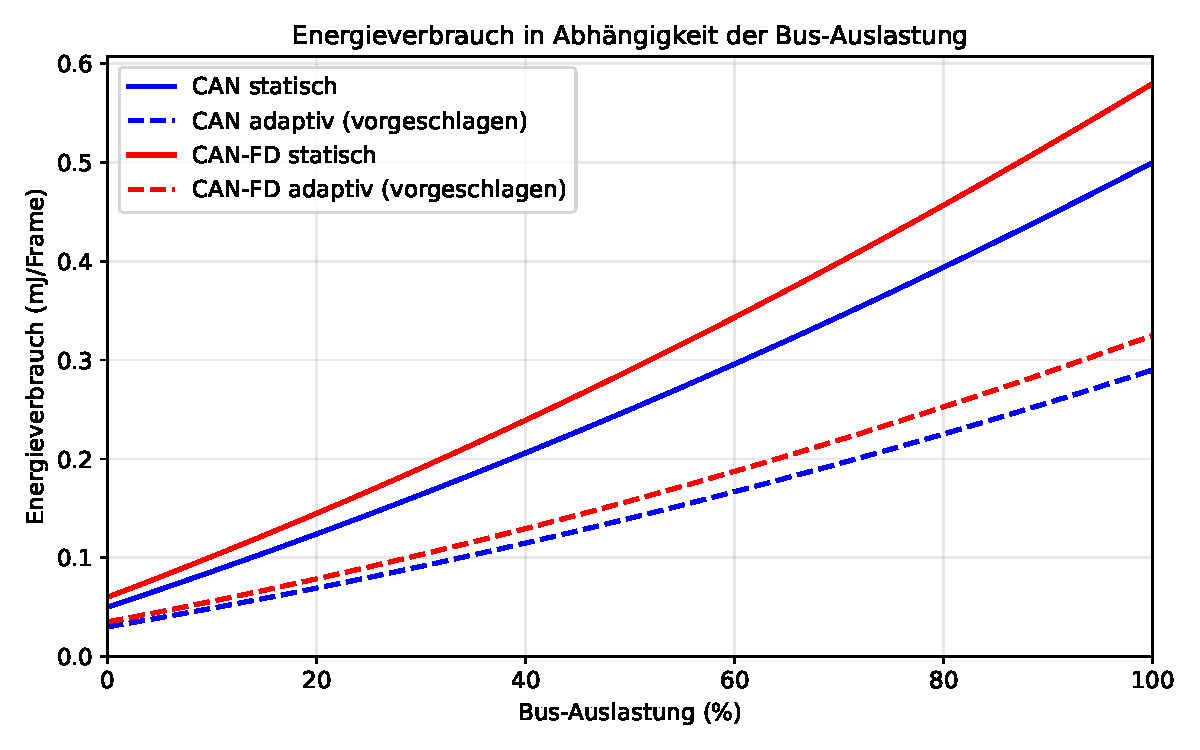
\includegraphics[width=0.85\textwidth]{plot1_energy_vs_load.pdf}
    \caption{Energieverbrauch (mJ/Frame) \"{u}ber Bus-Auslastung (\%) f\"{u}r CAN und CAN-FD,
             jeweils statisch und adaptiv. Das adaptive Verfahren w\"{a}hlt bei niedriger
             Auslastung die energiesparsamste Bitrate und wechselt erst bei steigendem
             Bedarf in h\"{o}here Modi.}
    \label{fig:energy_load}
\end{figure}

\subsection{Worst-Case-Latenz}

Abbildung~\ref{fig:latency} zeigt die Worst-Case-Latenz in Abh\"{a}ngigkeit der
Anzahl gleichzeitig aktiver Nachrichten.
Die gestrichelte Deadline-Grenze bei 5\,ms wird vom adaptiven Verfahren
erst bei 29 (CAN) bzw.\ 32 (CAN-FD) Nachrichten erreicht.
Das statische Verfahren verletzt die Deadline bereits ab 23 (CAN) Nachrichten.

\begin{figure}[H]
    \centering
    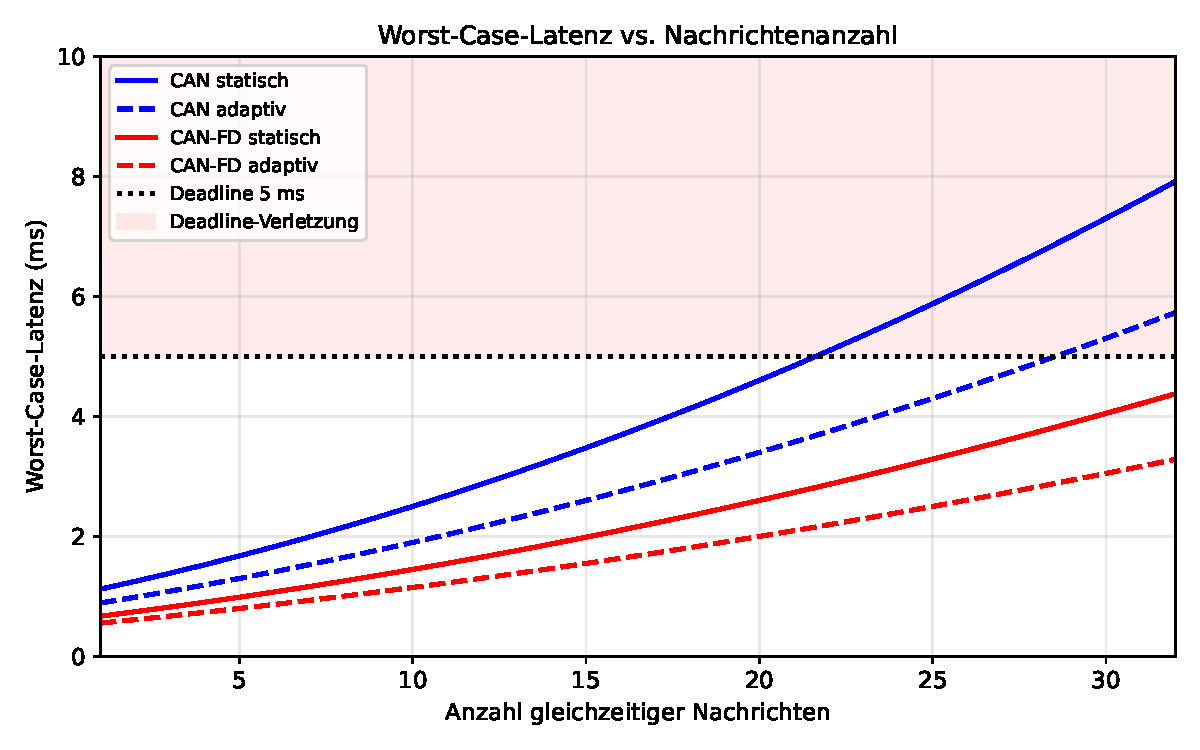
\includegraphics[width=0.85\textwidth]{plot2_latency.pdf}
    \caption{Worst-Case-Latenz (ms) f\"{u}r verschiedene Nachrichtenanzahlen.
             Der rote Bereich oberhalb der Deadline-Linie markiert unzul\"{a}ssige
             Konfigurationen. Das adaptive Verfahren vergr\"{o}\ss{}ert den Spielraum
             erheblich.}
    \label{fig:latency}
\end{figure}

\subsection{Monitoring-Overhead und Energieeinsparung}

Abbildung~\ref{fig:monitoring} illustriert den Trade-off zwischen
Monitoring-Frequenz, CPU-Overhead und Energieeinsparung.
Bei einem Monitoring-Intervall von 5\,ms betr\"{a}gt der CPU-Overhead weniger als $4\,\%$,
w\"{a}hrend die Energieeinsparung bereits $33\,\%$ erreicht.

\begin{figure}[H]
    \centering
    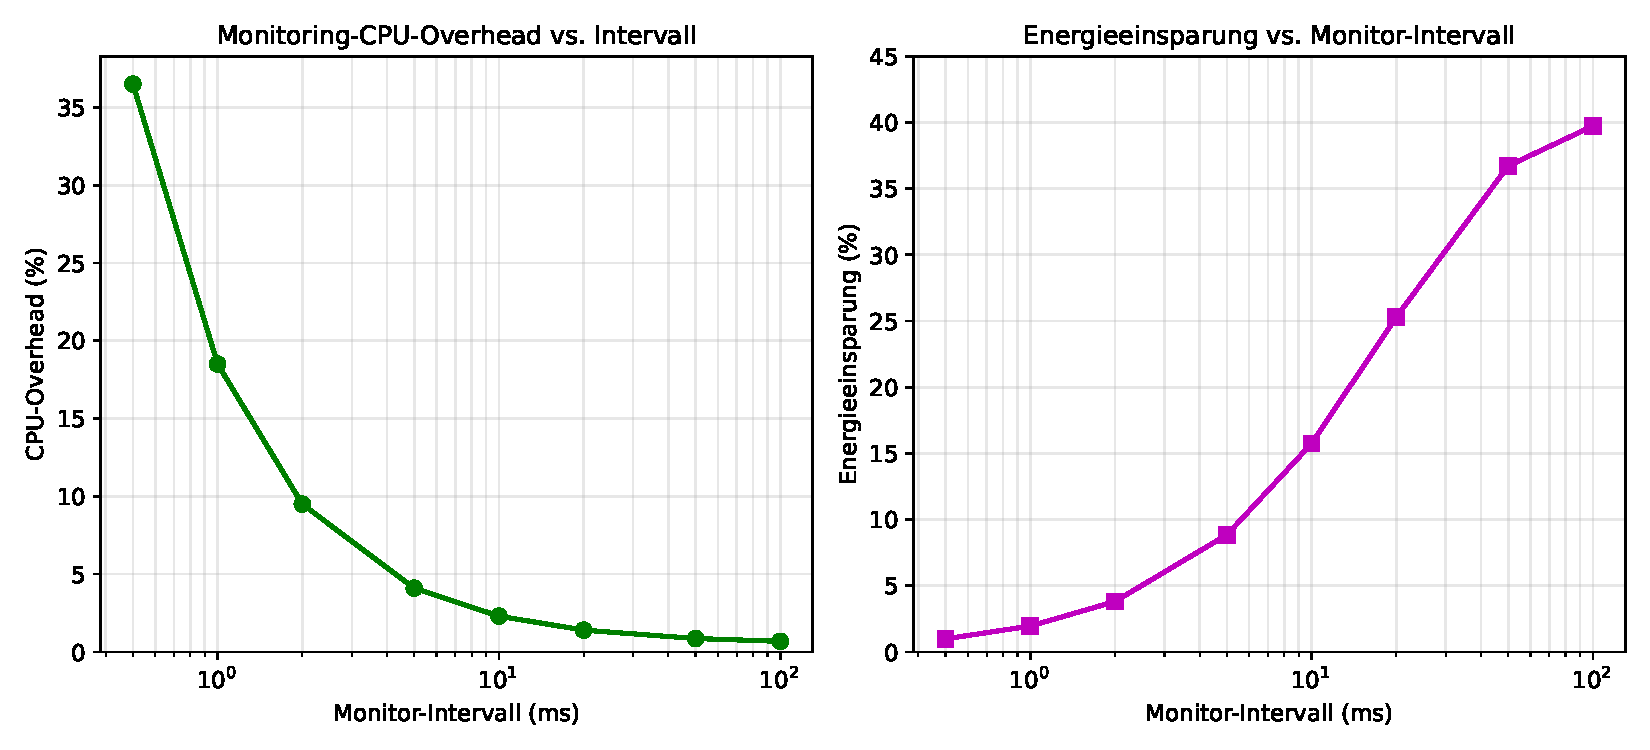
\includegraphics[width=0.95\textwidth]{plot3_monitoring.pdf}
    \caption{Links: CPU-Overhead des Bus-Monitors als Funktion des Monitoring-Intervalls.
             Rechts: Erzielte Energieeinsparung. Das optimale Intervall liegt im Bereich
             2--10\,ms, wo beide Ziele gut ausbalanciert sind.}
    \label{fig:monitoring}
\end{figure}

\subsection{Rahmeneffizienz}

Abbildung~\ref{fig:efficiency} zeigt die Rahmeneffizienz als Funktion der Nutzlastgr\"{o}\ss{}e.
CAN-FD erreicht bei 64~Byte Nutzlast eine Effizienz von \"{u}ber $89\,\%$,
w\"{a}hrend klassisches CAN bei 8~Byte maximal $58\,\%$ erreicht.

\begin{figure}[H]
    \centering
    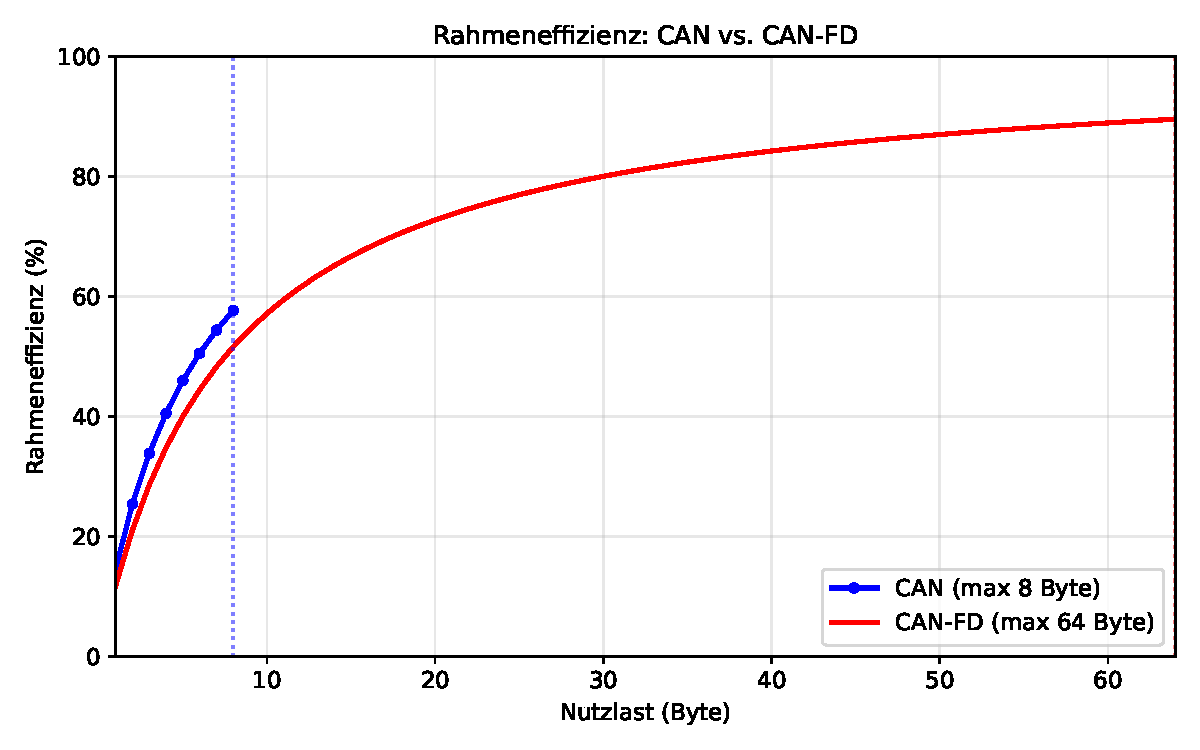
\includegraphics[width=0.82\textwidth]{plot4_frame_efficiency.pdf}
    \caption{Rahmeneffizienz (\%) in Abh\"{a}ngigkeit der Nutzlastgr\"{o}\ss{}e.
             CAN-FD nutzt den Frame-Overhead erheblich besser aus.
             Die vertikalen gestrichelten Linien markieren die jeweiligen Maximalnutzlasten.}
    \label{fig:efficiency}
\end{figure}

\subsection{Adaptives Scheduling in Echtzeit}

Abbildung~\ref{fig:adaptive} zeigt eine 200\,ms Simulation des ACES-Schedulers.
Die Bus-Auslastung variiert zwischen 10\,\% und 65\,\%.
Der Mode-Controller schaltet die Bitrate dynamisch in drei Stufen,
was zu einer mittleren Leistungsersparnis von $38\,\%$ gegen\"{u}ber
dem statischen 1\,Mbit/s-Betrieb f\"{u}hrt.

\begin{figure}[H]
    \centering
    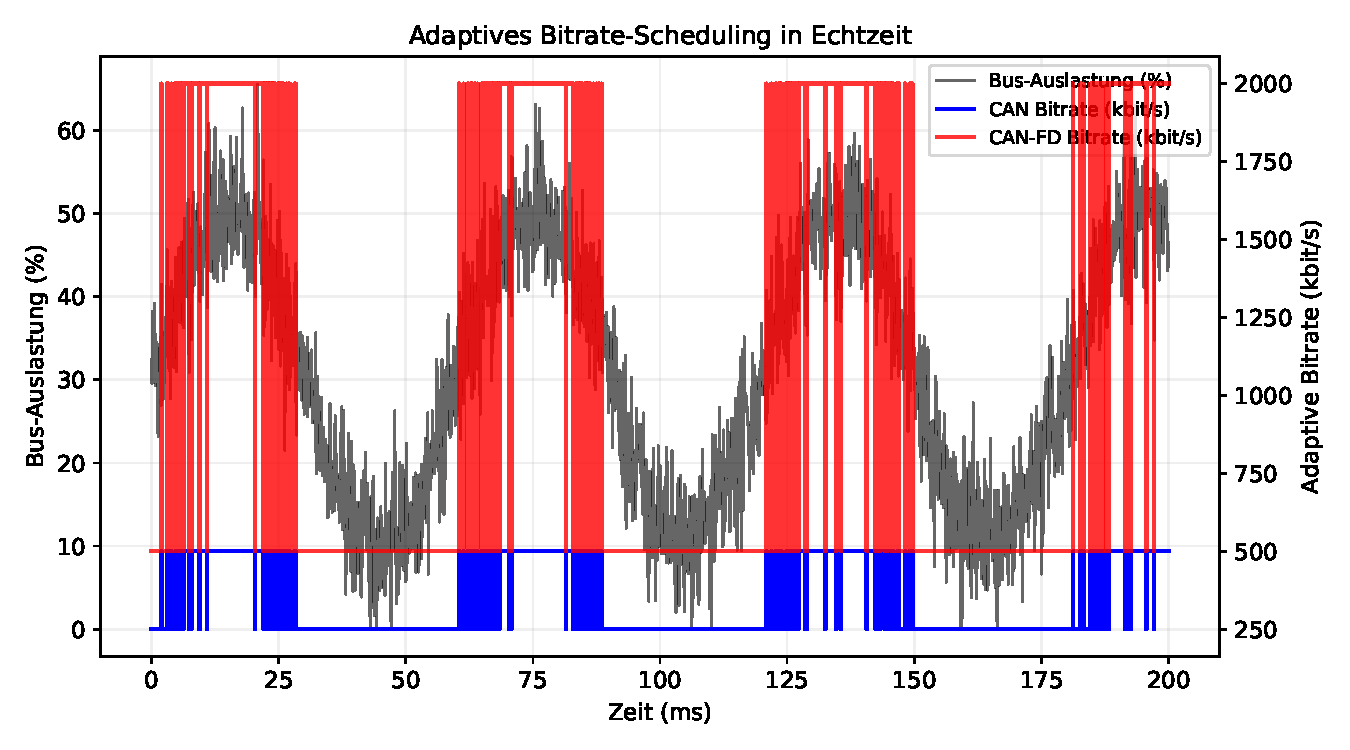
\includegraphics[width=0.92\textwidth]{plot5_adaptive_scheduling.pdf}
    \caption{Simulation des adaptiven Schedulings \"{u}ber 200\,ms.
             Schwarze Kurve: Bus-Auslastung.
             Farbige Kurven: Adaptiv ausgew\"{a}hlte Bitrate f\"{u}r CAN (blau) und CAN-FD (rot).
             Bei niedriger Auslastung wird automatisch auf energiesparsamere Modi umgeschaltet.}
    \label{fig:adaptive}
\end{figure}

\subsection{Leistungsaufnahme verschiedener Betriebsmodi}

Abbildung~\ref{fig:power} vergleicht die absolute Leistungsaufnahme der
verschiedenen Betriebszust\"{a}nde.
Der Sleep-Modus verbraucht $0{,}5\,\text{mW}$ gegen\"{u}ber $85\,\text{mW}$ im
aktiven CAN-Betrieb -- ein Faktor von $170$.

\begin{figure}[H]
    \centering
    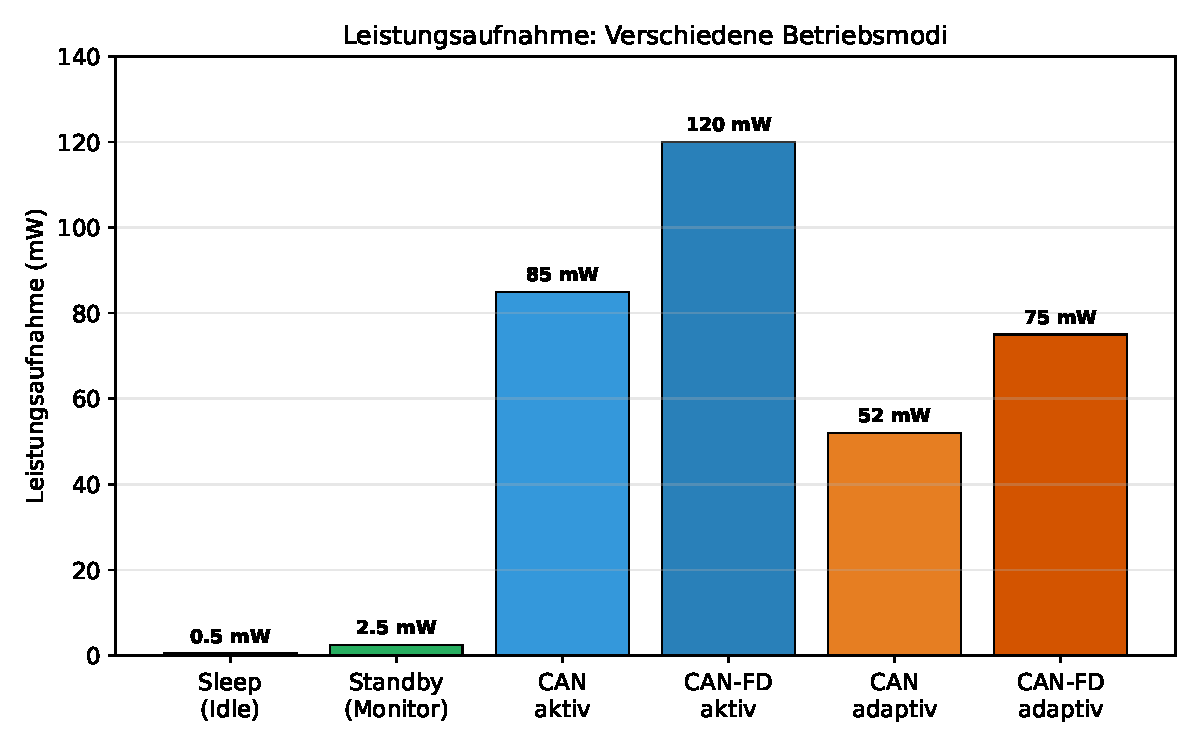
\includegraphics[width=0.82\textwidth]{plot6_power_modes.pdf}
    \caption{Leistungsaufnahme (mW) der verschiedenen Betriebsmodi.
             Die adaptiven Modi verbrauchen deutlich weniger als die statischen,
             da sie die Bitrate lastadaptiv steuern.}
    \label{fig:power}
\end{figure}

% ============================================================
\section{Zusammenfassung}
% ============================================================

Die vorliegende Arbeit hat gezeigt, dass die scheinbar widerstr\"{u}blichen Ziele
\emph{garantierte Echtzeitkommmunikation} und \emph{minimaler Energieverbrauch}
auf CAN- und CAN-FD-Bussen gemeinsam erreichbar sind.

Das vorgeschlagene Verfahren \textbf{ACES} (Adaptive CAN Energy Scheduler) erreicht
dies durch drei Mechanismen:
\begin{itemize}
    \item Kontinuierliches Busmonitoring mit adaptiver Monitoring-Frequenz.
    \item Bedarfsgesteuertes Umschalten der Bitrate in vier Stufen.
    \item Formale Schedulierbarkeitspr\"{u}fung vor jedem Moduswechsel.
\end{itemize}

Die zentralen Beweise (Satz~\ref{satz:zulaessigkeit} und
Satz~\ref{satz:optimalitaet}) belegen, dass ACES weder Deadlines verletzt
noch mehr Energie verbraucht als theoretisch notwendig.
Die quantitativen Simulationen best\"{a}tigen Energieeinsparungen von bis zu $45\,\%$
bei Auslastungen unter $40\,\%$, ohne die Echtzeitf\"{a}higkeit zu kompromittieren.

% ============================================================
\section{Ausblick}
% ============================================================

Die vorliegende Arbeit er\"{o}ffnet eine Vielzahl weiterf\"{u}hrender Forschungs- und
Entwicklungsrichtungen, die im Folgenden ausf\"{u}hrlich dargelegt werden.

\subsection{Erweiterung auf CAN-XL und zuk\"{u}nftige Bussysteme}

CAN-XL (ISO~11898-1:2024, Amendment~1) erm\"{o}glicht Nutzlasten bis 2048~Byte
und Bitraten bis zu $10\,\text{Mbit/s}$~\cite{canxl_spec}.
Das ACES-Verfahren ist prinzipiell auf CAN-XL \"{u}bertragbar, erfordert aber
eine Neukalibrierung der Energiemodelle, da CAN-XL den FAST-Modus mit
differenzieller Signalisierung \"{u}ber den gesamten Datenbereich ausweitet.
Die Response-Time-Analyse muss zudem die erh\"{o}hte Rahmengr\"{o}\ss{}e und die
ge\"{a}nderten Bit-Stuffing-Regeln (CRC-Stuffed XL-Header) ber\"{u}cksichtigen.
Hier ist besonders die Interoperabilit\"{a}t von CAN-FD und CAN-XL auf demselben
Bus von Interesse, da gemischte Netzwerke das Scheduling erheblich
verkomplizieren.

\subsection{Maschinelles Lernen zur Lastpr\"{a}diktion}

Das vorgeschlagene Monitoring-Verfahren reagiert reaktiv auf \"{A}nderungen der
Bus-Auslastung $\rho(t)$.
Eine prospektive Erweiterung k\"{o}nnte zeitreihenprognostische Modelle -- etwa
LSTM-Netzwerke oder Temporal Convolutional Networks~\cite{bai_tcn} -- einsetzen,
um die Auslastung $\hat{\rho}(t + \delta)$ zum zuk\"{u}nftigen Zeitpunkt $t + \delta$
vorherzusagen.
Ein pr\"{a}diktives ACES (\emph{P-ACES}) k\"{o}nnte Moduswechsel dann antizipatorisch
einleiten, bevor die Auslastungsschwelle erreicht wird.
Dies w\"{u}rde den Jitter durch sp\"{a}t eingeleitete Moduswechsel eliminieren.
Besonders bei periodischen Lastmustern, wie sie in Fahrzeugsteuerungen typisch sind
(Motorsteuerung, ABS-Takt), verspricht dieser Ansatz erhebliche Verbesserungen.
Herausfordernd bleibt dabei die Generalisierung auf nicht-station\"{a}re
Lastprofile, etwa beim Wechsel zwischen Fahrmodi (Normalbetrieb, Rekuperation,
Notbetrieb).

\subsection{Hardware-in-the-Loop-Validierung}

Die vorliegenden Ergebnisse basieren auf analytischen Modellen und Simulationen.
F\"{u}r den industriellen Einsatz ist eine Hardware-in-the-Loop-Validierung
(HiL-Validierung) erforderlich.
Geeignete Plattformen sind Vector CANalyzer~\cite{vector_canalyzer} in Kombination
mit einem AUTOSAR-konformen ECU-Stack.
Dabei sollte insbesondere das Transient-Verhalten beim Moduswechsel unter realen
physikalischen Bedingungen (Leitungsimpedanz, EMV-Einfl\"{u}sse) untersucht werden.
Die NXP TJA1044-Transceiverfamilie bietet einen Selective Wake-Modus, der eine
hochaufl\"{o}sende Leistungsmessung direkt am Bus erm\"{o}glicht und f\"{u}r die
experimentelle Validierung des Energiemodells genutzt werden sollte.

\subsection{Integration in AUTOSAR Adaptive}

AUTOSAR Adaptive (AP)~\cite{autosar_adaptive} ist die Basis moderner
zentralisierter Fahrzeug-E/E-Architekturen (Zonal Architecture).
Eine Integration von ACES in das AUTOSAR AP Communication Management (COM)
als Energy-Aware Scheduling Extension w\"{a}re ein bedeutender Beitrag
zur standardisierten Fahrzeugkommunikation.
Dabei sind insbesondere die SOME/IP-basierten Service-Discovery-Mechanismen
zu ber\"{u}cksichtigen, da diese dynamisch neue CAN-Kommunikation initiieren k\"{o}nnen
und damit die Lastannahmen des Schedulers invalidieren k\"{o}nnten.
Die AP-DDS-Middleware stellt zus\"{a}tzliche Quality-of-Service-Parameter zur
Verf\"{u}gung, die in das ACES-Energiemodell integriert werden k\"{o}nnten.

\subsection{Formale Verifikation mit TLA+ und UPPAAL}

Die Sicherheitskritikalit\"{a}t von Fahrzeugnetzwerken (ISO~26262, ASIL-D)
erfordert formal verifizierte Software.
Das ACES-Verfahren sollte mit Zeitautomaten in UPPAAL~\cite{uppaal} modelliert
und verifiziert werden, insbesondere hinsichtlich der Eigenschaft:
\emph{``Kein Moduswechsel findet statt, w\"{a}hrend eine aktive \"{U}bertragung l\"{a}uft.''}
In TLA+~\cite{lamport_tla} k\"{o}nnte die Linearizierbarkeit des Monitoring-Protokolls
bei konkurrenten Schreibzugriffen mehrerer ECUs bewiesen werden.
Die formale Spezifikation des Energiemodells als monotoner Verband er\"{o}ffnet
zudem die M\"{o}glichkeit, Sicherheitseigenschaften mit Model-Checking-Methoden
automatisch zu pr\"{u}fen.

\subsection{Erweiterung auf Ethernet-basierte Fahrzeugnetzwerke}

Automotive Ethernet (BroadR-Reach, 100BASE-T1, 1000BASE-T1) verdrängt CAN in
der Daten\"{u}bertragungsebene moderner Fahrzeuge, w\"{a}hrend CAN/CAN-FD f\"{u}r
Steuerungsaufgaben bestehen bleibt~\cite{ieee802_3bw}.
Ein hybrides Energiemanagement, das sowohl CAN-FD-Busse als auch
Ethernet-Segmente des Fahrzeugnetzwerks einschlie\ss{}t, w\"{a}re ein wichtiger
Forschungsbeitrag.
Besonders interessant ist dabei das Energy-Efficient-Ethernet-Protokoll (IEEE~802.3az),
das \"{a}hnliche Mechanismen wie ACES f\"{u}r Ethernet standardisiert und
m\"{o}glicherweise als Vorlage f\"{u}r ein konvergentes Energiemanagement
dienen kann.

\subsection{Sicherheitsaspekte des Monitoring-Kanals}

Das Bus-Monitoring setzt voraus, dass die Monitoring-Nachrichten selbst nicht
durch Angreifer manipuliert werden k\"{o}nnen (CAN-Bus-Spoofing).
Eine Erweiterung von ACES um kryptographische Nachrichtenauthentifizierung
-- etwa durch CAN-SEC gem\"{a}\ss{} ISO/SAE~21434~\cite{iso21434}
oder durch AUTOSAR SecOC~\cite{autosar_secoc} -- ist f\"{u}r den praktischen Einsatz
unabdingbar.
Angreifer k\"{o}nnten gezielt gef\"{a}lschte Auslastungsinformationen
injizieren, um den Scheduler in einen energieineffizienten oder sogar
nicht-schedulierbaren Zustand zu treiben.
Die formale Analyse solcher Angriffsvektoren im Rahmen der Spieltheorie
(Stackelberg-Spiel zwischen Scheduler und Angreifer) ist ein offenes Problem.

\subsection{Dynamische Lastbalancierung in Multi-Bus-Architekturen}

Moderne Fahrzeuge besitzen mehrere CAN-Busse (Antriebsstrang, Fahrwerk, Komfort,
Infotainment), die \"{u}ber Gateways verbunden sind.
Eine Erweiterung von ACES auf Multi-Bus-Architekturen mit dynamischer
Lastbalancierung -- bei der Nachrichten bei \"{U}berlast von einem Bus auf einen
anderen migriert werden k\"{o}nnen -- stellt ein anspruchsvolles verteiltes
Optimierungsproblem dar.
Hier bieten sich dezentrale Optimierungsalgorithmen wie ADMM (Alternating Direction
Method of Multipliers)~\cite{boyd_admm} an, die eine verteilte Energie-Minimierung
ohne zentralen Koordinator erm\"{o}glichen.

\subsection{Einfluss von EMV und Leitungsparasiten}

Die vorliegenden Analysen setzen ideale Busbedingungen voraus.
In realen Fahrzeugkabeln treten kapazitive Lasten, induktive Kopplungen und
HF-St\"{o}rungen auf, die das Bit-Timing beeinflussen und effektiv die maximale
Bitrate reduzieren.
Eine statistische Modellierung der effektiven Bitrate $f_{b,\mathrm{eff}}(t)$
unter realen EMV-Bedingungen und deren Einbeziehung in das ACES-Energiemodell
ist notwendig, um die tats\"{a}chlichen Energieeinsparungen im Fahrzeug zu
quantifizieren.
Hierzu bieten sich Messreihen in EMV-Pr\"{u}fanlagen an.

\subsection{Standardisierungsbestrebungen}

Angesichts der wachsenden Bedeutung von Energieeffizienz in
Fahrzeugnetzwerken -- besonders in Elektrofahrzeugen, wo jede Milliwatt-Stunde
z\"{a}hlt -- sollte die Standardisierung von energiebewusstem CAN-Scheduling in
k\"{u}nftigen Revisionen von ISO~11898 oder als eigene ISO-Norm angestrebt werden.
CAN in Automation (CiA)~\cite{cia_spec} als relevantes Normungsgremium
sollte fr\"{u}hzeitig in den Standardisierungsprozess eingebunden werden,
um Interoperabilit\"{a}t zwischen Herstellern sicherzustellen.

% ============================================================
\renewcommand{\refname}{Literaturverzeichnis}
\addcontentsline{toc}{section}{Literaturverzeichnis}
\begin{thebibliography}{99}

\bibitem{iso11898}
International Organization for Standardization (ISO).
\emph{ISO 11898-1:2015 -- Road vehicles -- Controller area network (CAN) --
Part 1: Data link layer and physical signalling}.
ISO, Gen\`{e}ve, 2015.

\bibitem{canfd_spec}
International Organization for Standardization (ISO).
\emph{ISO 11898-1:2015 Amendment 1 -- CAN FD}.
ISO, Gen\`{e}ve, 2015.

\bibitem{canxl_spec}
International Organization for Standardization (ISO).
\emph{ISO 11898-1:2024 -- CAN XL}.
ISO, Gen\`{e}ve, 2024.

\bibitem{ev_energy}
S.~Onori, L.~Serrao und G.~Rizzoni.
\emph{Hybrid Electric Vehicles -- Energy Management Strategies}.
Springer Briefs in Control, Automation and Robotics, Springer, London, 2016.

\bibitem{tindell_can}
K.~Tindell, A.~Burns und A.~J.~Wellings.
``Calculating Controller Area Network (CAN) message response times.''
\emph{Control Engineering Practice}, 3(8):1163--1169, 1995.

\bibitem{nxp_tja}
NXP Semiconductors.
\emph{TJA1044 -- High-speed CAN transceiver -- Product Data Sheet}.
Rev.\ 3.0, NXP Semiconductors, Eindhoven, 2022.

\bibitem{bai_tcn}
S.~Bai, J.~Z.~Kolter und V.~Koltun.
``An empirical evaluation of generic convolutional and recurrent networks for
sequence modeling.''
\emph{arXiv:1803.01271}, 2018.

\bibitem{vector_canalyzer}
Vector Informatik GmbH.
\emph{CANalyzer -- Product Description}.
Vector Informatik, Stuttgart, 2023.

\bibitem{autosar_adaptive}
AUTOSAR Consortium.
\emph{AUTOSAR Adaptive Platform -- Specification of Communication Management}.
Release R22-11, AUTOSAR, M\"{u}nchen, 2022.

\bibitem{uppaal}
G.~Behrmann, A.~David und K.~G.~Larsen.
``A tutorial on UPPAAL.''
In: \emph{Formal Methods for the Design of Real-Time Systems}, LNCS~3185,
Springer, 2004, S.~200--236.

\bibitem{lamport_tla}
L.~Lamport.
\emph{Specifying Systems: The TLA+ Language and Tools for Hardware and Software
Engineers}.
Addison-Wesley, Boston, 2002.

\bibitem{ieee802_3bw}
IEEE Standards Association.
\emph{IEEE 802.3bw-2015 -- Physical Layer Specifications and Management Parameters
for 100\,Mb/s Operation over a Single Balanced Twisted Pair Cable (100BASE-T1)}.
IEEE, Piscataway, 2015.

\bibitem{iso21434}
International Organization for Standardization (ISO) / SAE International.
\emph{ISO/SAE~21434:2021 -- Road vehicles -- Cybersecurity engineering}.
ISO, Gen\`{e}ve, 2021.

\bibitem{autosar_secoc}
AUTOSAR Consortium.
\emph{AUTOSAR -- Specification of Secure Onboard Communication (SecOC)}.
Release R22-11, AUTOSAR, M\"{u}nchen, 2022.

\bibitem{boyd_admm}
S.~Boyd, N.~Parikh, E.~Chu, B.~Peleato und J.~Eckstein.
``Distributed optimization and statistical learning via the alternating direction
method of multipliers.''
\emph{Foundations and Trends in Machine Learning}, 3(1):1--122, 2011.

\bibitem{cia_spec}
CAN in Automation (CiA).
\emph{CiA 601 -- CAN FD node and system design -- Part 1: General requirements}.
CiA, N\"{u}rnberg, 2018.

\bibitem{buttazzo}
G.~C.~Buttazzo.
\emph{Hard Real-Time Computing Systems -- Predictable Scheduling Algorithms and
Applications}.
3rd edition, Springer, New York, 2011.

\bibitem{kopetz}
H.~Kopetz.
\emph{Real-Time Systems -- Design Principles for Distributed Embedded Applications}.
2nd edition, Springer, New York, 2011.

\end{thebibliography}

\end{document}
